%%%%%%%%%%%%%%%%%%%%%%%%%%%%%
\chapter{Implementazione}
%%%%%%%%%%%%%%%%%%%%%%%%%%%%%
\section{Struttura dell'applicazione e ambiente di sviluppo}
Come detto nel capitolo 3, per la stesura dell'applicazione ho deciso di impiegare due editor diversi in virtù delle loro differenze. Il primo, IntelliJ, è stato utilizzato per strutturare il backend, il supporto nativo a Spring lo ha reso una facile scelta.
\\
Ho costruito lo scheletro del progetto utilizzando il tool open source spring initializr\footnote{\url{https://start.spring.io/}} che consente di creare una configurazione iniziale, tra le opzioni di personalizzazione vi sono: la versione del framework Spring boot, la versione di Java, la tipologia di progetto (Gradle\footnote{
Gradle è un sistema open source per l'automazione dello sviluppo fondato sulle idee di Apache Ant e Apache Maven, che introduce un domain-specific language (DSL) basato su Groovy, al posto della modalità XML usata da Apache Maven per dichiarare la configurazione del progetto. Gli script Gradle possono essere eseguiti direttamente, in contrasto con le definizioni dei progetti Apache Maven (pom.xml).\cite{GradleDef}
} o Maven\footnote{
In informatica Apache Maven è uno strumento di gestione di progetti software basati su Java e build automation.\cite{MavenDef}
}) e le dipendenze di base incluse nel progetto.
\\
Le librerie che sono andato ad utilizzare sono le seguenti:
\begin{itemize}
    \item Lombok: Libreria che mette a disposizione dei programmatori annotazioni semplici che sostituiscono costruttori, getter e setter e altre utilities indispensabili per il corretto funzionamento di una classe\footnote{
    Sostituisce il già ottimo sistema di generazione del codice di IntelliJ, il miglioramento risiede nell'eleganza della soluzione, si impiegano infatti delle annotazioni al posto di righe e righe di codice standard. Questo incrementa di molto la leggibilità.
    }.
    \item Spring Web: Libreria che consente di ricevere e gestire richieste HTTP.
    \item Spring security: Libreria che consente di mettere in campo sistemi di controllo di autenticazioni e autorizzazioni.
    \item MySQL driver: driver che gestisce la connessione tra database e applicazione Spring.
    \item Spring data JPA: libreria che astrae le complessità di gestione delle operazioni con il database
    \item Java e-mail sender: Libreria che consente la costruzione e l'invio di email.
    \item Spring Cloud Gateway: Libreria che consente di strutturare un Application Gateway.
    \item Java JWT: Utile libreria per abilitare l'utilizzo di JSON Web Token per l'autorizzazione delle azioni richieste dagli utenti.
\end{itemize}
Per quanto riguarda il frontend ho utilizzato l'editor Visual Studio Code, per le ragioni esposte in precedenza. ReactJS si appoggia a node, dunque, dopo l'installazione di node è stato possibile lanciare il comando.
\begin{lstlisting} [language=bash]
$ npm create-react-app nome-progetto
\end{lstlisting}
Il comando da terminale, una volta terminata l'esecuzione, produce una cartella che contiene un boiler-plate da cui partire per produrre il proprio progetto React.
\\
Così come Spring, anche React aveva la necessità di includere una serie di package per estendere le capacità del framework, le librerie che ho dovuto includere nel progetto sono le seguenti:
\begin{itemize}
    \item react-pdf/renderer: Ottima libreria open source per la gestione, visualizzazione e generazione di pdf a partire da codice JSX.
    \item reduxjs/toolkit: Libreria per la gestione di stati globali.
    \item react-router-dom: Libreria che consente di associare a indirizzi testuali delle componenti React.
    \item react-images-uploading: Libreria React che consente di gestire il caricamento di immagini da parte degli utenti.
    \item redux-persist: Libreria che astrae la gestione del local storage per redux.
    \item styled-components: Libreria che consente di definire componenti React di puro stile che sono dunque prive di logica.
\end{itemize}



%%%%%%%%%%%%%%%%%%%%%%%%%%%%%
\section{Backend}
%%%%%%%%%%%%%%%%%%%%%%%%%%%%%
In questa sezione andrò ad esplorare un po' più nel dettaglio quali siano state le scelte implementative lato backend.
\subsection{Struttura del Backend}
Per ciascun microservizio (escluso il Gateway che agisce semplicemente da firewall) ho riutilizzato sempre la stessa struttura:
\begin{itemize}
    \item Models: Che sono i modelli delle entità coinvolte nell'applicazione, la definizione di questi modelli era necessaria per poter sfruttare pienamente le capacità di Hibernate\footnote{Hibernate mappa le classi Java in tables del database}.
    \item Controllers: Che si occupano di gestire le richieste provenienti dall'esterno andando a mappare una specifica richiesta con una funzione offerta da un service.
    \item Services: Classi che offrono una serie di funzioni che possono essere richiamate dai controller e che si occupano di implementare la logica effettiva dell'applicazione.
    \item Repositories: Classi che definiscono i repository necessari per la gestione dell'applicazione e che includono al loro interno eventuali funzioni che vengono mappate in query personalizzate.
\end{itemize}
Oltre a questi elementi ho aggiunto due componenti per quel che riguarda la sezione di security:
\begin{itemize}
    \item jwt: Una serie di classi personalizzate che servono a generare il token per gli utenti e a controllarne la validità in fase di autorizzazione.
    \item securityConfig: Una serie di classi volte a definire le security policies implementate.
\end{itemize}
A tutte le classi facenti parte dei domini sopra elencati sono state associate delle annotazioni che ne consentono la gestione efficace e l'immediato riconoscimento da parte dell'engine di Spring.
\begin{figure}[h]
    \centering
    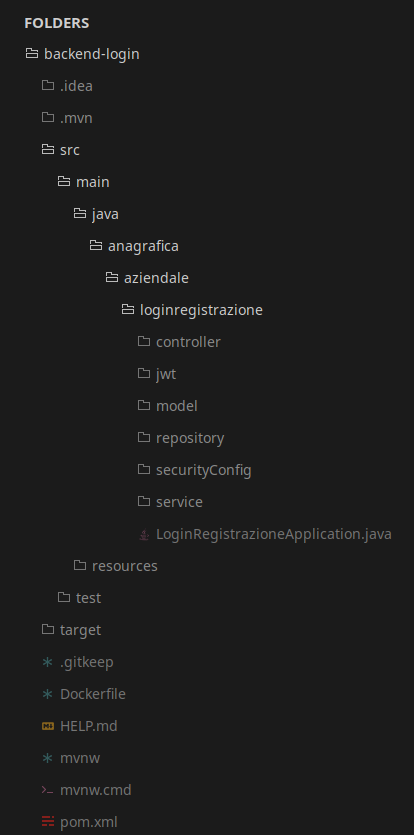
\includegraphics[height=300px]{./images/security_filesystem.png}
    \caption{La struttura del microservizio di sicurezza}
    \label{fig:micSecurity}
\end{figure}

%%%%%%%%%%%%%%%%%%%%%%%%%%%%%
\subsection{Configurazione dell'immagine}
%%%%%%%%%%%%%%%%%%%%%%%%%%%%%
Come si può vedere dall'immagine \ref{fig:micSecurity}, il microservizio di login contiene un Dockerfile, che è un file di configurazione dell'immagine che verrà poi caricata dentro il container di Docker.
\\
Ciascun microservizio ha un suo Dockerfile e volevo concentrarmi in particolare sul modello che ho impiegato per poter gestire il backend. Come dicevo nel capitolo 2, uno degli obiettivi che mi sono posto per la composizione dell'applicazione è quello di consentire a chiunque di costruire l'intera struttura impiegando un unico comando da terminale ovvero:
\begin{lstlisting} [language=bash]
$ docker compose up
\end{lstlisting}
Dunque, come si può vedere dal codice in figura \ref{fig:dockerfile}, il Dockerfile è diviso in due sezioni: la prima consente di creare un singolo file Jar a partire dall'operazione di maven install; nella seconda il file jar viene spostato all'interno del container, di modo che venga effettivamente creato il point of entry per il microservizio.
\\
\begin{figure}[h]
    \centering
    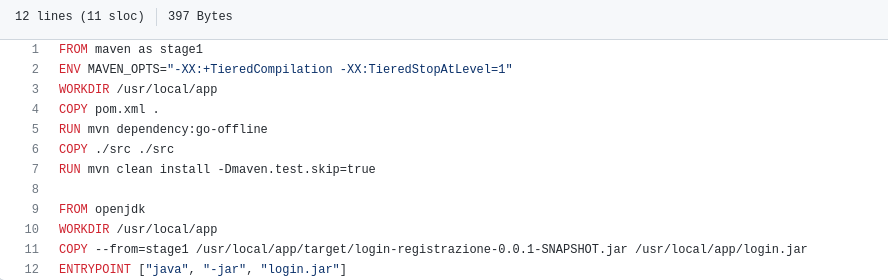
\includegraphics[width=450px, height=150px]{./images/security_dockerfile.png}
    \caption{Il Dockerfile associato al microservizio di sicurezza}
    \label{fig:dockerfile}
\end{figure}
Il motivo per cui il Dockerfile è strutturato in questo modo, anzichè una più semplice configurazione, è il fatto che se avessi inserito le sole righe 9 - 12 sarei stato obbligato ad eseguire lo step di costruzione del file jar manualmente da linea di comando o dall'interfaccia di IntelliJ.
\\
Inoltre la build in due stadi, come precedentemente affermato nel capitolo 2, mi consente di diminuire la dimensione dei container evitando che questi contengano cose inutili. Maven, infatti, non servirà più una volta che il processo di build sarà stato completato. Dunque conviene impiegarlo solo all'inizio e poi lasciarlo fuori dall'immagine in modo che non occupi spazio.



%%%%%%%%%%%%%%%%%%%%%%%%%%%%%
\section{Frontend}
%%%%%%%%%%%%%%%%%%%%%%%%%%%%%
Per quello che riguarda il frontend ho cercato il più possibile di essere fedele alla logica di sviluppo in ReactJS, dunque era importante cercare di rendere il più possibile riusabili le componenti.
\\
L'applicazione consiste di 50 componenti. Ne ho calcolato la dimensione media, in righe di codice, ed è venuto fuori che il numero medio è di 104.2. Tra tutte le componenti il 72\% di queste è lunga meno di 100 righe, solo l'8\% del totale invece si è rivelato di lunghezza superiore a 300 righe, si tratta infatti solo di alcuni file contenenti una serie di funzioni che mi sarebbe convenuto dividere per rendere più netta la differenza delle responsabilità.

\begin{figure}[h]
    \centering
    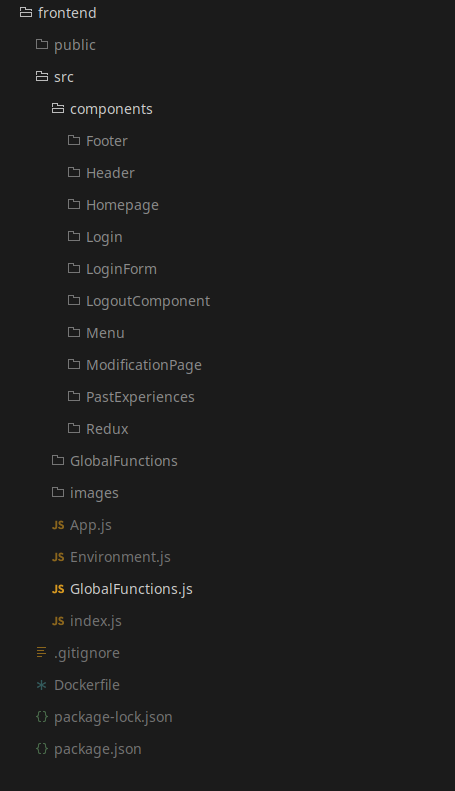
\includegraphics[width=200px, height=350px]{./images/frontend_filesystem.png}
    \caption{La struttura del microservizio di frontend}
    \label{fig:frontend}
\end{figure}



%%%%%%%%%%%%%%%%%%%%%%%%%%%%%
\section{Interfaccia utente}
%%%%%%%%%%%%%%%%%%%%%%%%%%%%%
Per l'interfaccia grafica mi sono fatto tentare da alcuni stili preimpostati offerti da AdminLTE\footnote{
Un sito che offre template open source da inserire in progetti frontend per strutturare delle interfacce utente / admin.\cite{AdminLTE}
}, sui quali sono poi andato a mettere le mani per renderli più vicini al design aziendale, che usa principalmente: bianco, antracite e blu per gli accenti.

%%%%%%%%%%%%%%%%%%%%%%%%%%%%%
\subsection{Login}
%%%%%%%%%%%%%%%%%%%%%%%%%%%%%
La pagina di login, mostrata in figura \ref{fig:loginPage}, è quella con cui si interfaccia chiunque utilizzi l'applicazione, oltre alla sezione di inserimento delle proprie credenziali vi è un header in alto che è quello che viene visualizzato in qualsiasi altra pagina.
\\
Per poter accedere alle funzionalità offerte è prima necessario autenticarsi tramite la propria email e la propria password.
\\
Dopo che il bottone di "SIGN IN" è stato premuto i dati vengono inoltrati al backend e vengono eseguite le operazioni mostrate nella sezione dedicata ai diagrammi di sequenza.

\begin{figure}[h]
    \centering
    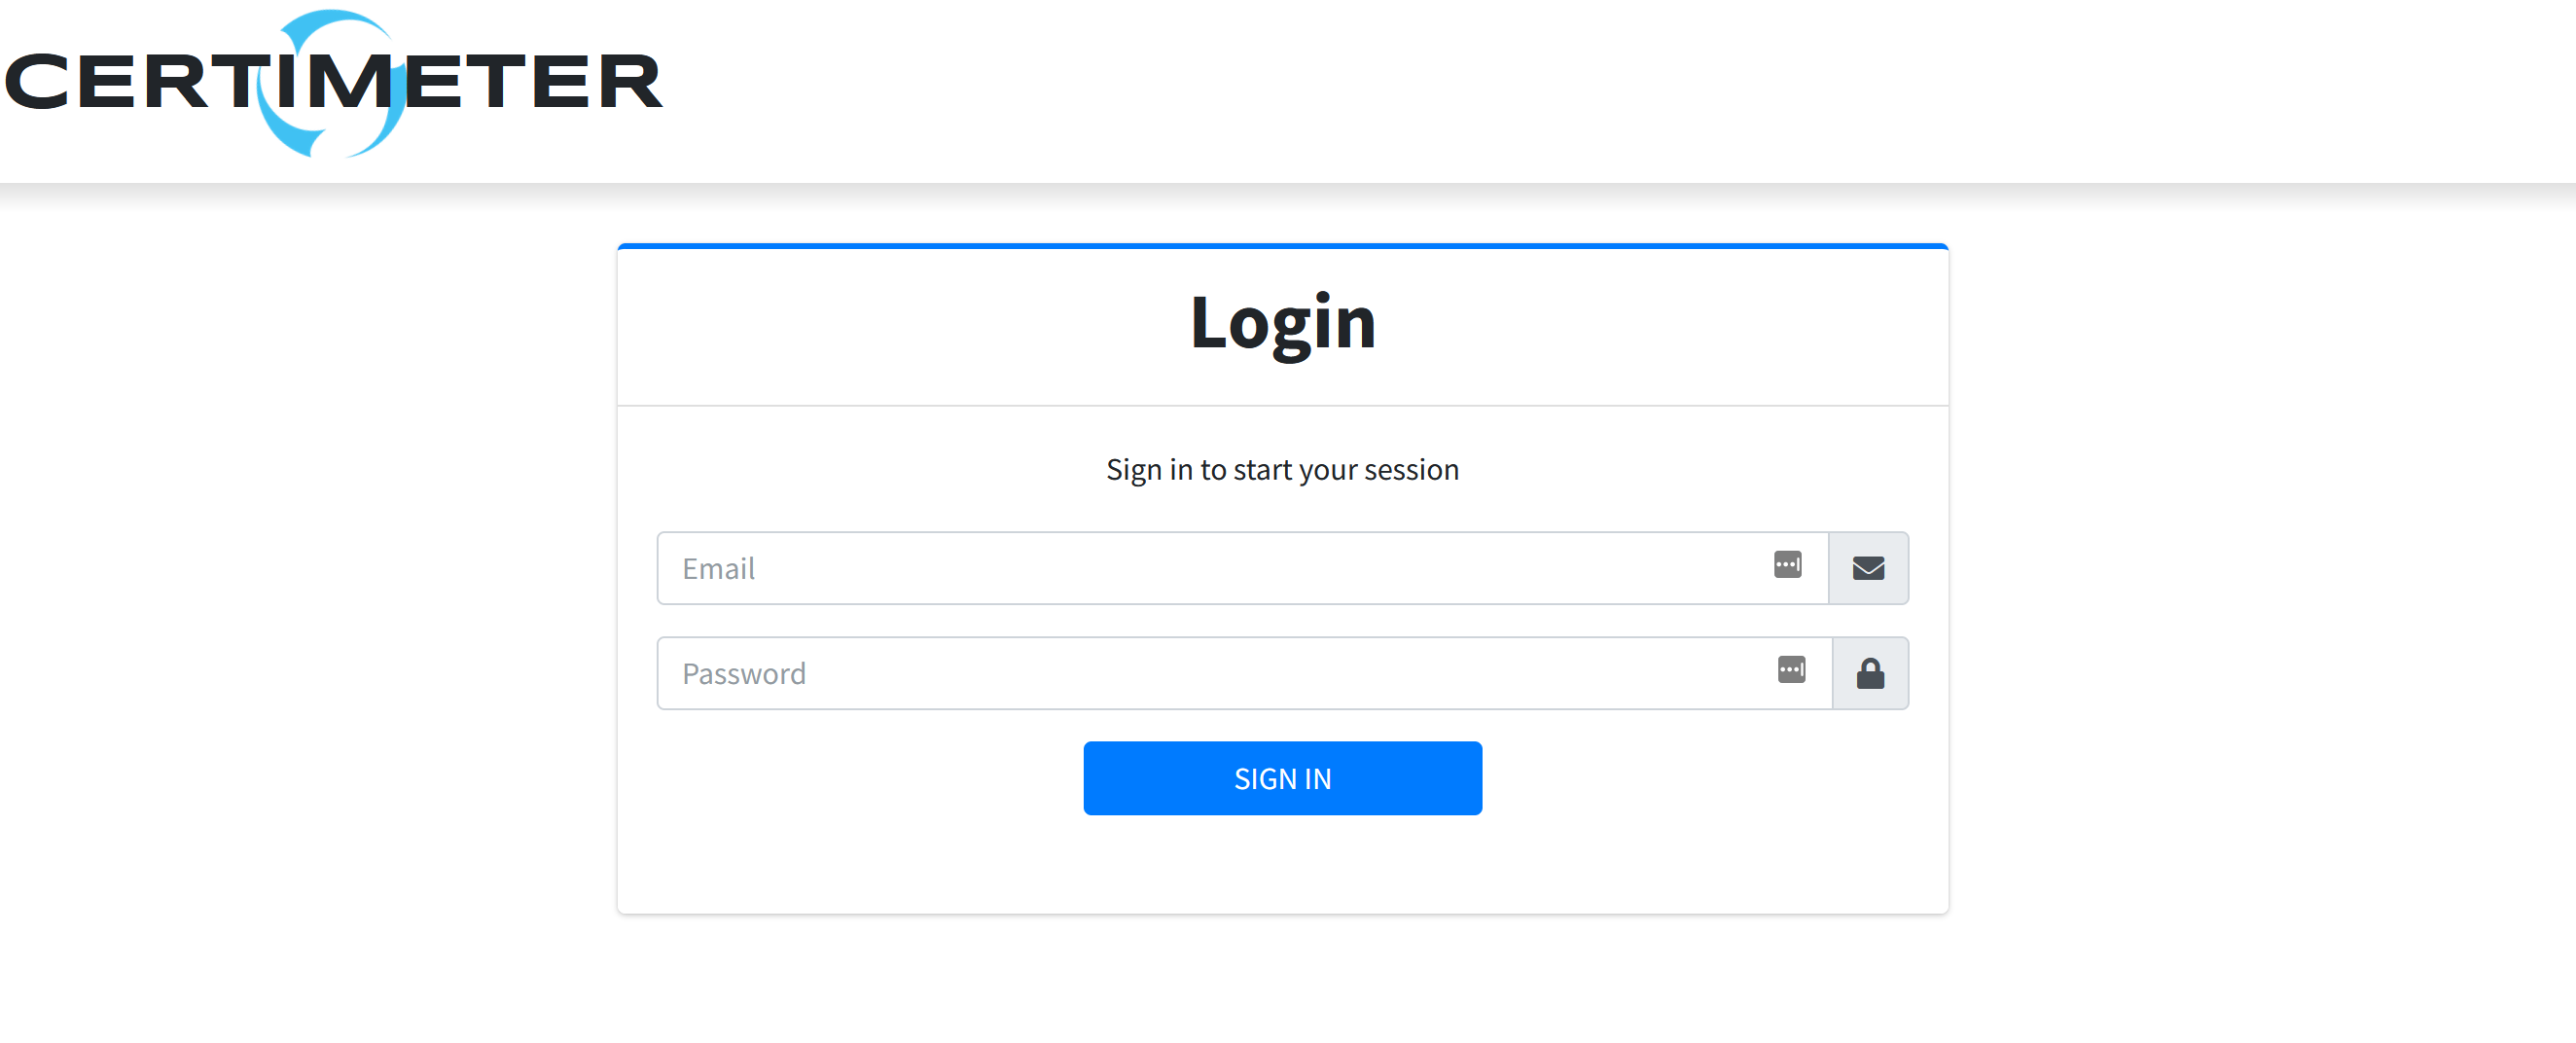
\includegraphics[width=450px]{./images/login_component.png}
    \caption{Struttura della componente di Login}
    \label{fig:loginPage}
\end{figure}

%%%%%%%%%%%%%%%%%%%%%%%%%%%%%
\subsection{Homepage}
%%%%%%%%%%%%%%%%%%%%%%%%%%%%%
La homepage è l'unica pagina, oltre a quella di login, presente all'interno del sistema, un esempio è visibile in figura \ref{fig:homepage}.
\\
Questa contiene un menu sidebar a sinistra\footnote{
Inserito a posteriori su consiglio del capo
}, che concede l'accesso a tutte le altre funzionalità previste, e il resto dello schermo è occupato da una card che conterrà tutti i vari elementi del menu. Non appena si entra nell'applicazione si è accolti dalla visualizzazione di default, che è quella contenente i dati personali dell'utente e la sua foto profilo. \footnote{
In figura \ref{fig:homepage} il caso di esempio è quello di un utente admin del sistema
}
\\
La struttura della homepage viene mantenuta tra i vari utenti, l'unica cosa che cambia, sono le voci della sidebar di sinistra. Per l'admin tali voci sono:
\begin{itemize}
    \item Il proprio profilo, identificato dall'immagine profilo, il nome e il cognome scritti in maiuscolo.
    \item Le proprie skills, identificate dalla voce skills.
    \item Le proprie esperienze pregresse, identificate dalla voce Experiences, queste saranno divise in esperienze da consulente ed esperienze lavorative.
    \item Il proprio curriculum, generato automaticamente dal sistema, nella sezione Curriculum Pdf.
    \item Il menu di modifica delle proprie informazioni, identificato da Information update, per l'utente è sostanzialmente tutto modificabile tranne alcune informazioni che ho considerato immodificabili perchè tendono a non cambiare (nome, cognome ed email).
    \item Le funzioni di admin, identificate dalla voce Admin Functions.
    \item La funzione di Logout.
\end{itemize}
Per l'utente comune la sidebar è identica, a meno della voce Admin Functions, per ovvie ragioni.

\begin{figure}[h]
    \centering
    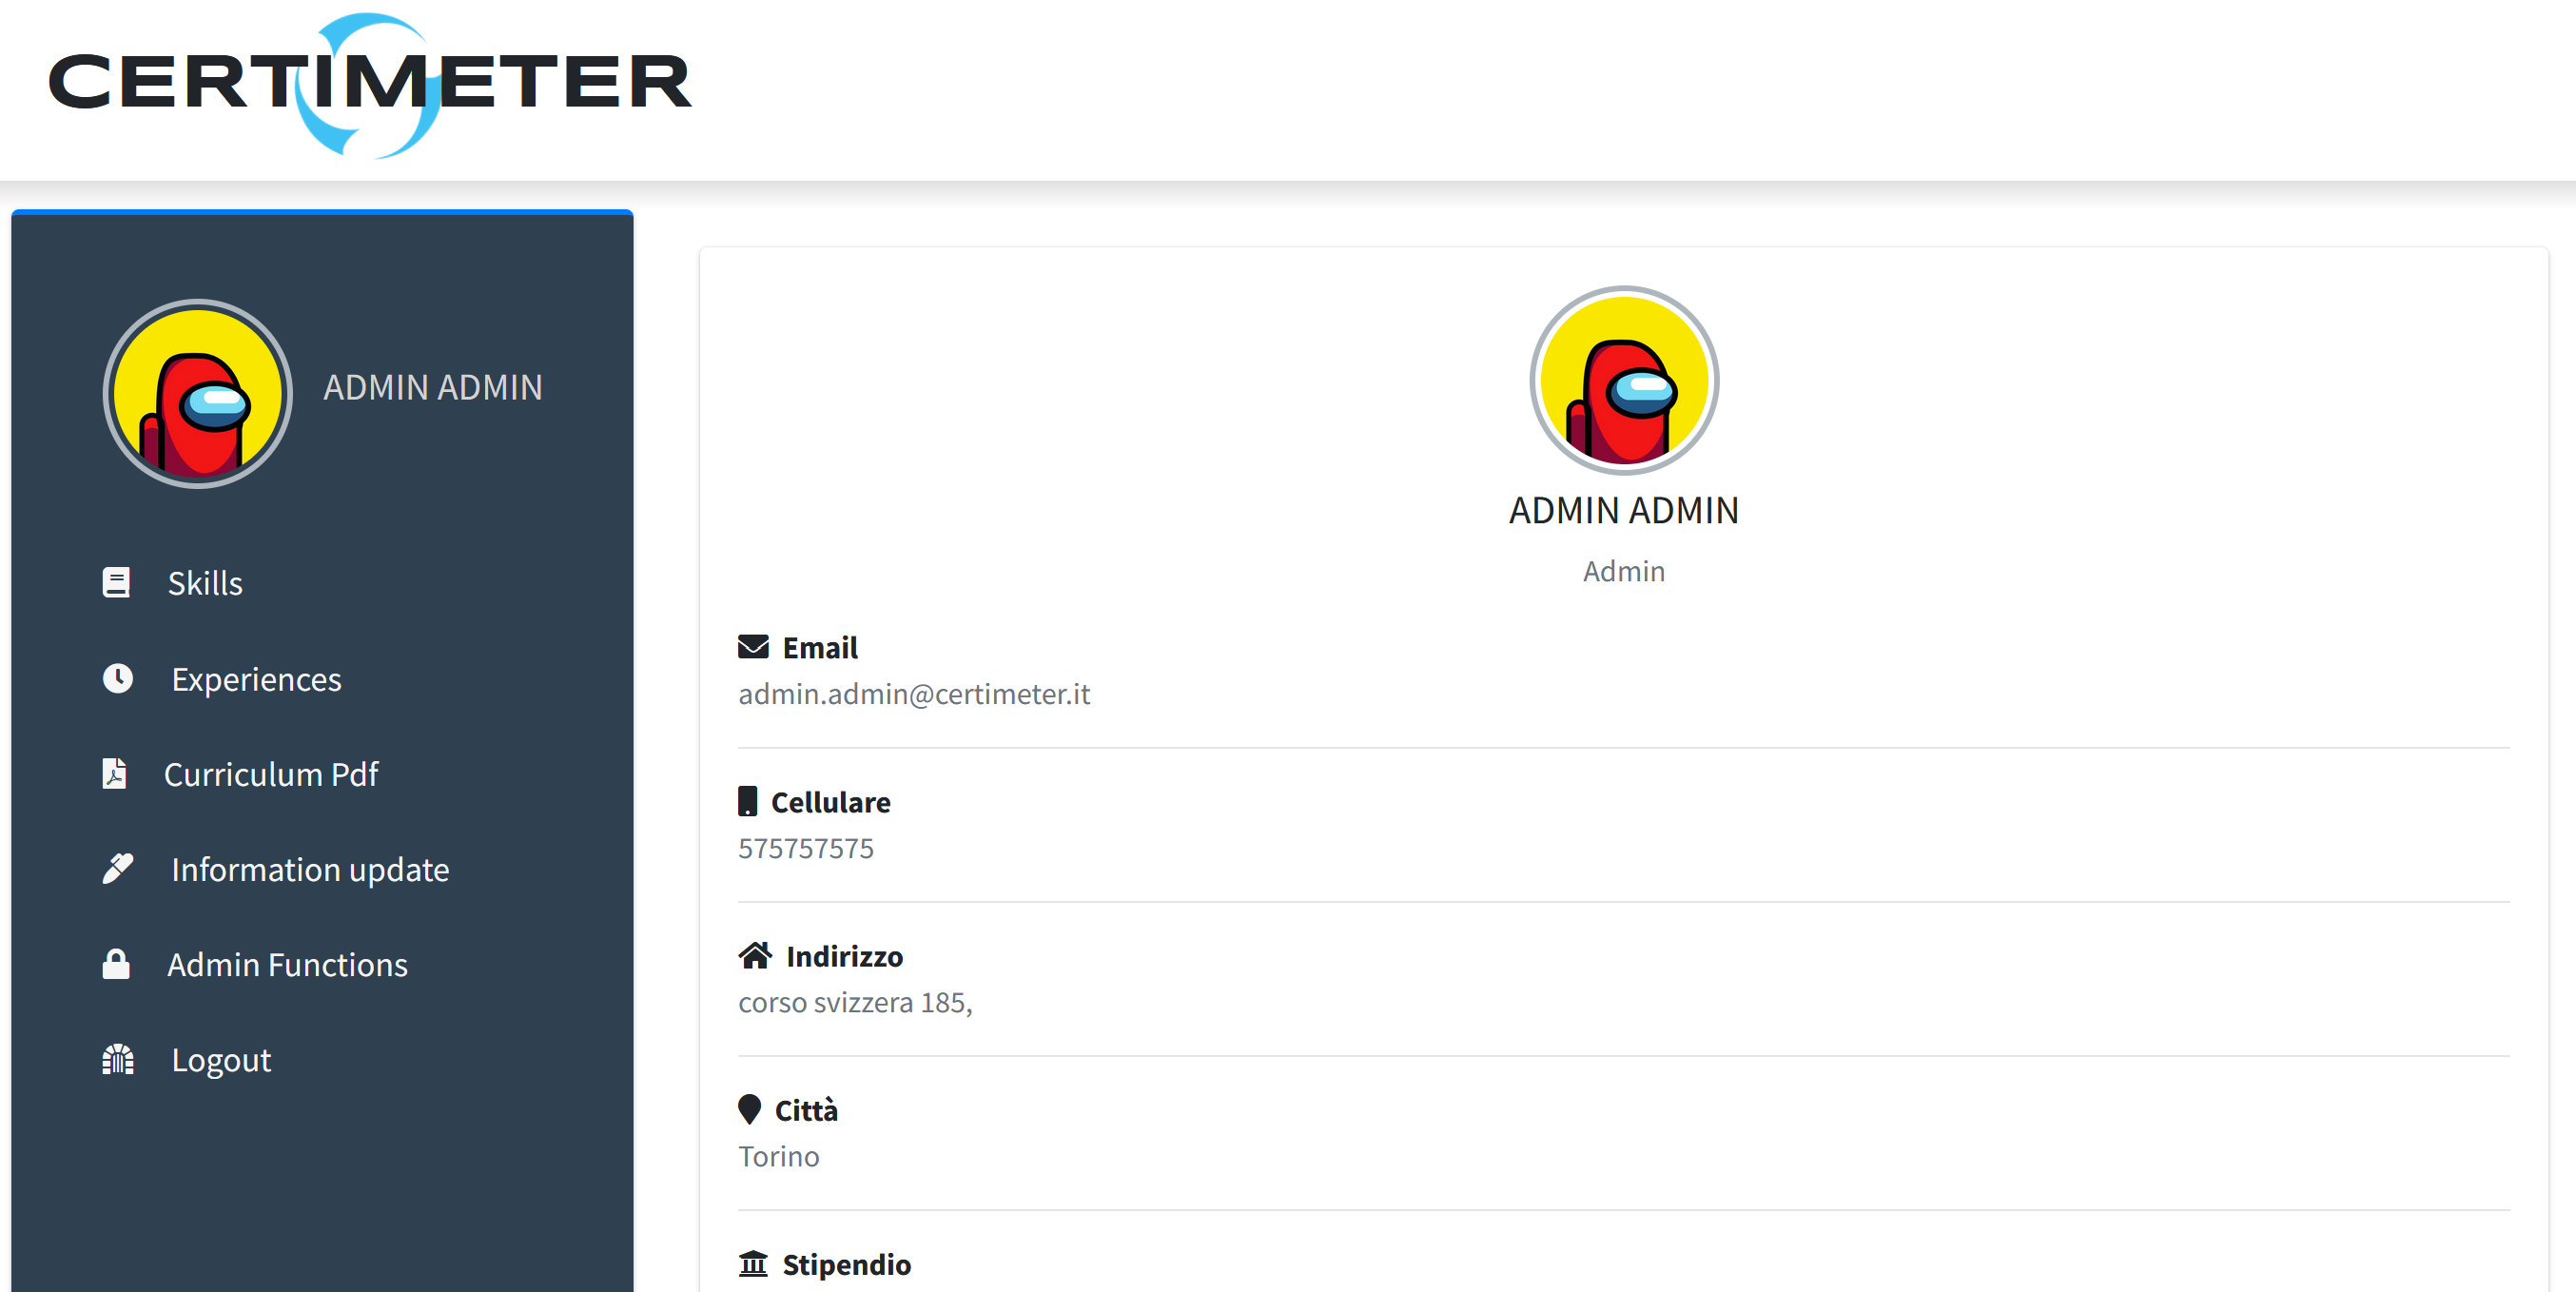
\includegraphics[width=450px]{./images/homepage.png}
    \caption{Struttura della homepage}
    \label{fig:homepage}
\end{figure}

%%%%%%%%%%%%%%%%%%%%%%%%%%%%%
\subsection{Skills section}
%%%%%%%%%%%%%%%%%%%%%%%%%%%%%
Nella sezione di visualizzazione delle skill, mostrata in figura \ref{fig:skillVisualization}, ho optato per un grafico a barre che raffronta la lunghezza della barra con un valore che va da 1 a 5\footnote{
Non ho incluso il valore 0 per il semplice fatto che, siccome le skill sono autovalutate, se l'utente può valutare una skill come 0 equivale a non averla.
} e che rappresenta il livello di padronanza che l'utente ritiene di avere rispetto a una determinata skill.
\\
Le skill sono state raggruppate in tre categorie:
\begin{itemize}
    \item Hard Skill: le skill concettuali e teoriche, ho pensato di includere in questa categoria i linguaggi di programmazione e i framework più noti.
    \item Soft Skill: le skill che riguardano l'ambito più umano (competitività, teamwork, etc...).
    \item Office suite skills: le skill leagate ai programmi di office più noti, conoscenze spesso richieste in ambito aziendale.
\end{itemize}
Riguardo alla selezione delle skill si faccia riferimento alla sezione di information update.

\begin{figure}[h]
    \centering
    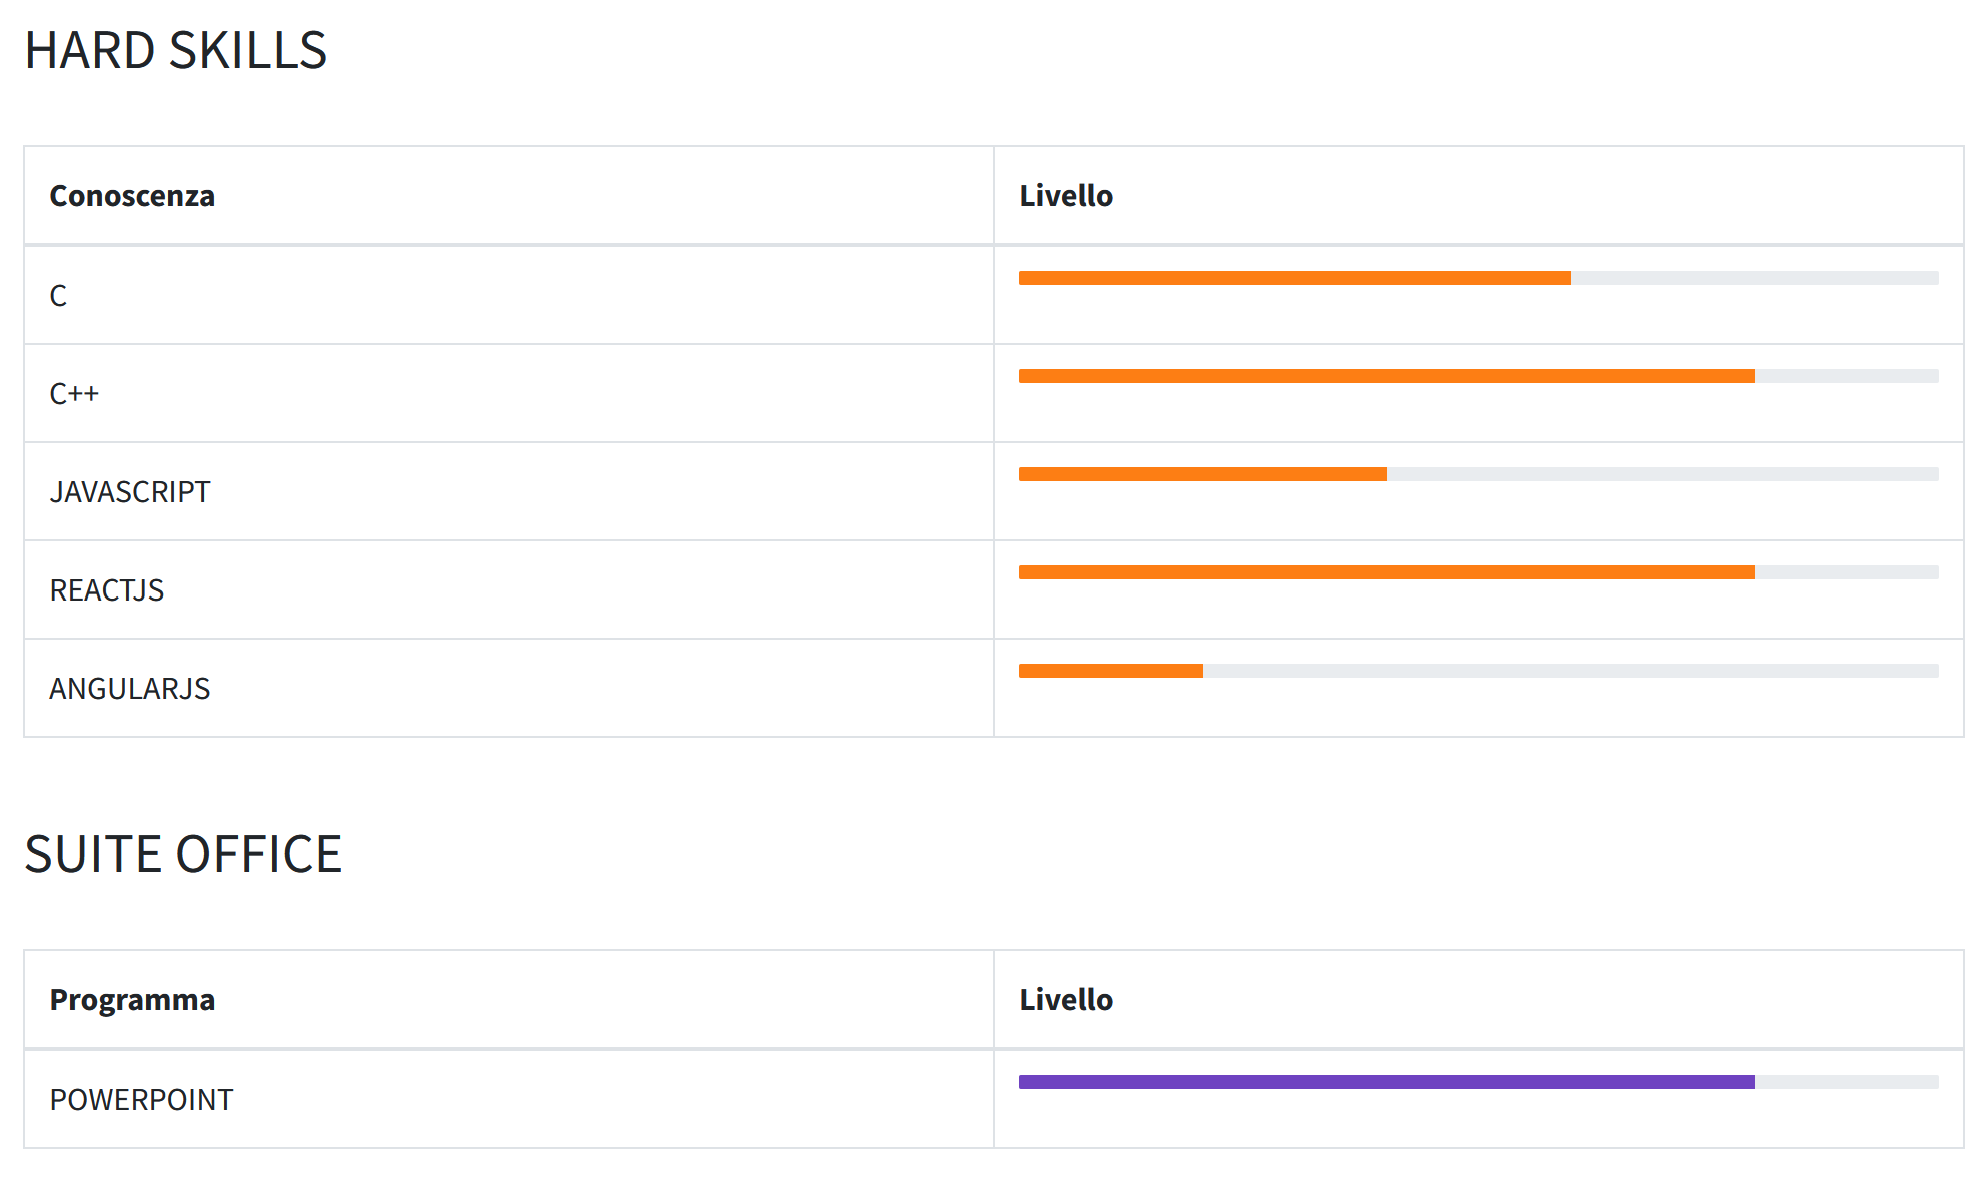
\includegraphics[width=450px]{./images/skills.png}
    \caption{Struttura della sezione delle skills}
    \label{fig:skillVisualization}
\end{figure}

%%%%%%%%%%%%%%%%%%%%%%%%%%%%%
\subsection{Curriculum Pdf}
%%%%%%%%%%%%%%%%%%%%%%%%%%%%%
Per la sezione di curriculum Pdf, mostrata in figura \ref{fig:curriculum}, ho inserito all'interno della card il sistema di visualizzazione e salvataggio dei pdf incorporato nel browser. Il curriculum fa un sommario di quelle che sono le informazioni presenti all'interno dello stato di ReactJS e le riproduce utilizzando una visualizzazione che è simile a quella proposta nel resto dell'applicazione.
\\
Per assemblare la visualizzazione ho dovuto usare una sintassi particolare ideata dal gruppo dietro al framework react-pdf/renderer. La sintassi è JSX ma vengono forniti dei componenti preimpostati a cui possono essere poi associati degli stili CSS specifici per renderli personalizzati.
\\
\'E inoltre possibile, tramite l'utilizzo del pulsante di fullscreen di passare a una visualizzazione del pdf che occupa lo schermo intero.

\begin{figure}[h]
    \centering
    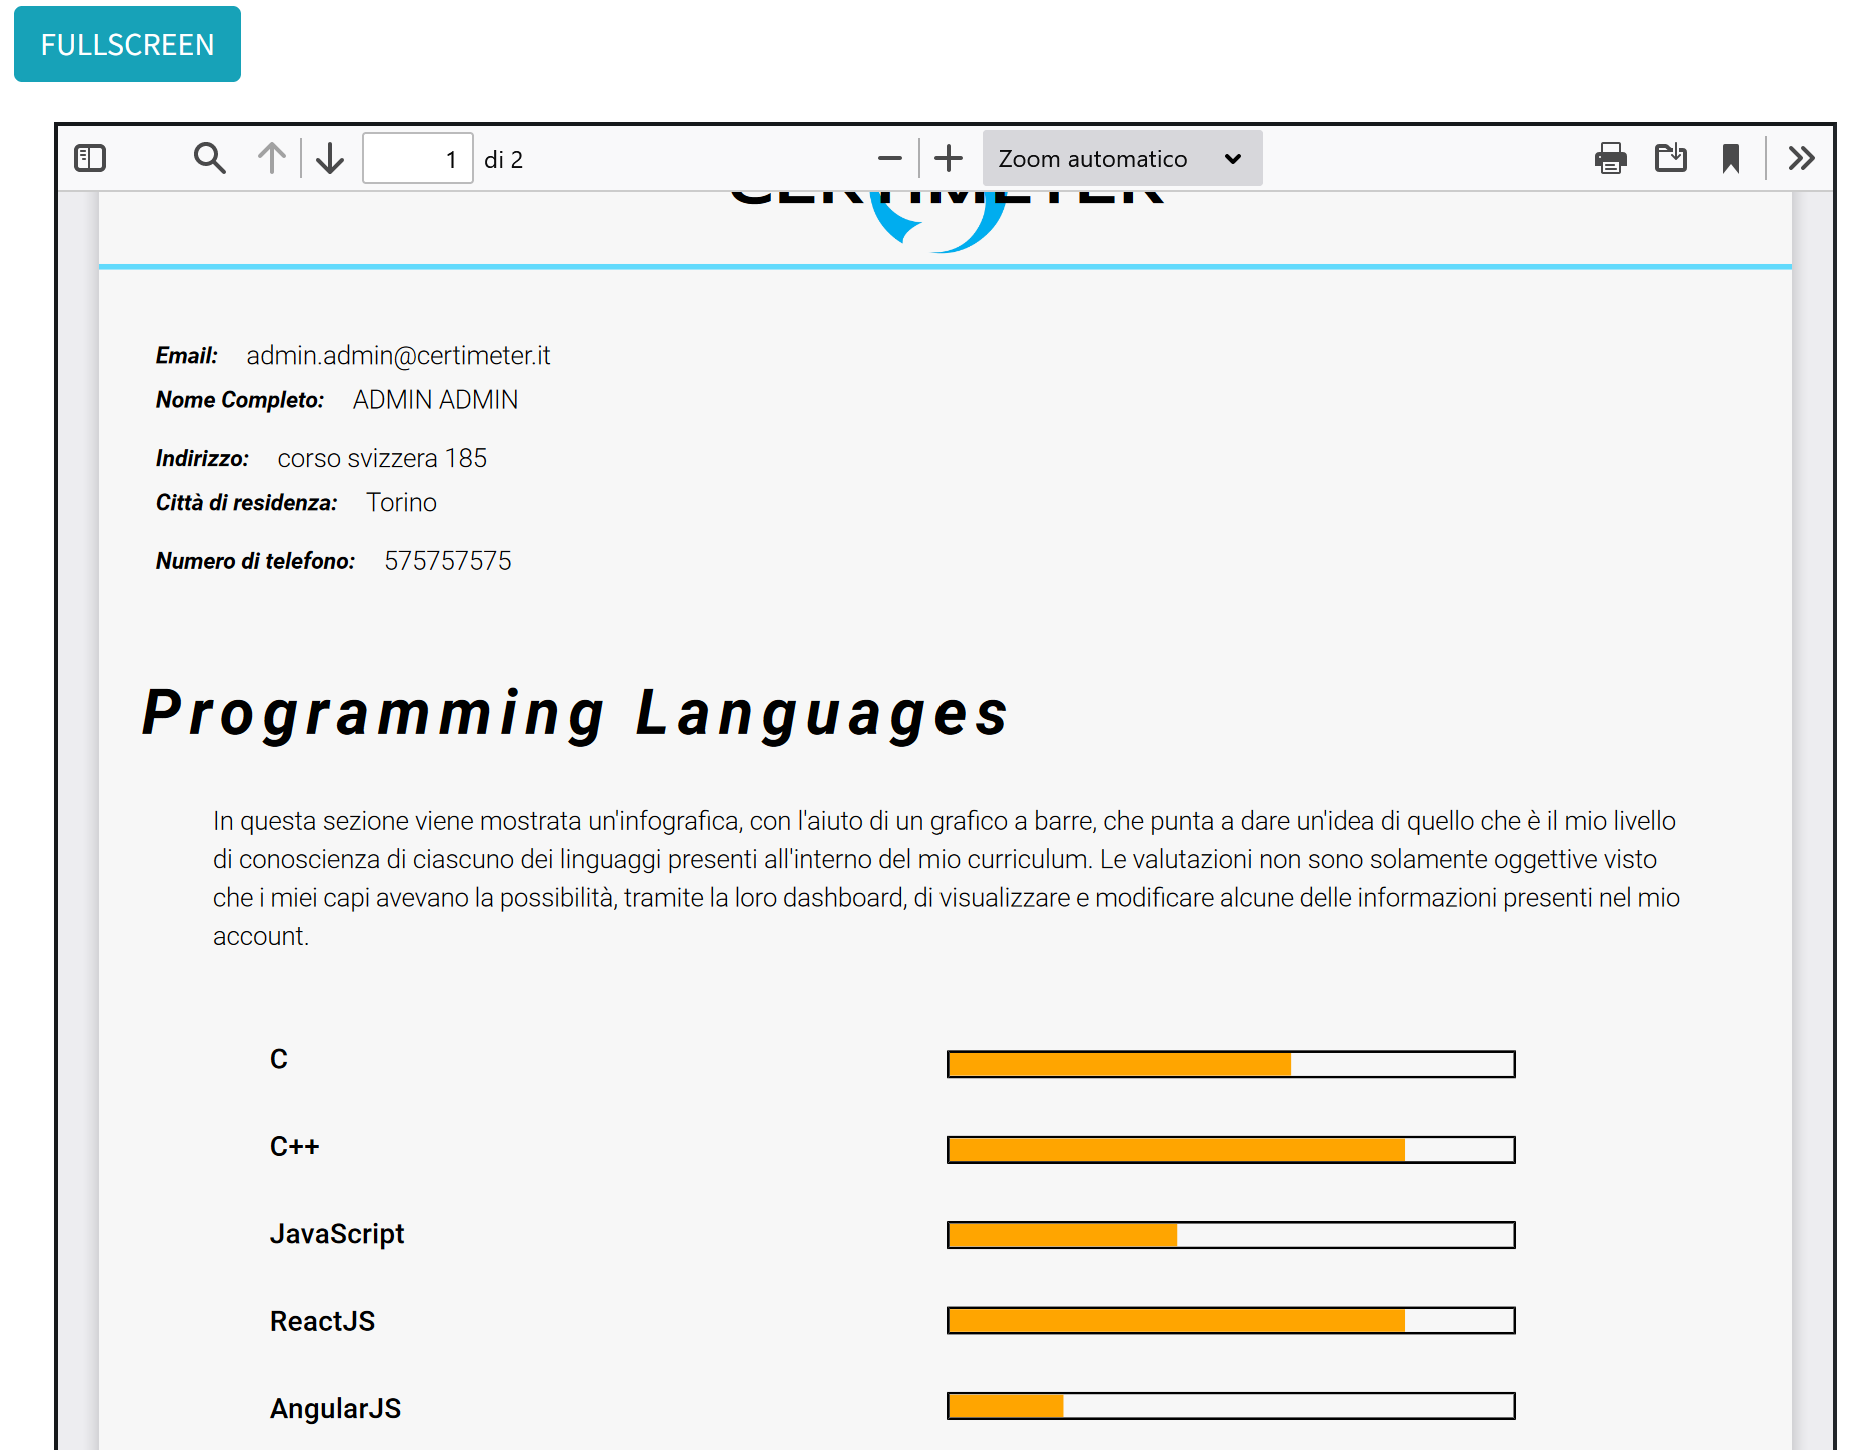
\includegraphics[width=450px]{./images/pdf.png}
    \caption{Sezione di visualizzazione del pdf}
    \label{fig:curriculum}
\end{figure}

%%%%%%%%%%%%%%%%%%%%%%%%%%%%%
\subsection{Information update}
%%%%%%%%%%%%%%%%%%%%%%%%%%%%%
La sezione di information update apre una card che contiene un sottomenu all'interno del quale sono presenti tutte le possibili operazioni che un utente può compiere. \'E possibile passare da una visualizzazione all'altra premendo sul nome corrispondente nell'header mostrato nella parte alta di figura \ref{fig:modificaInformazioni}. Di default la pagina aperta sarà quella di modifica delle informazioni personali.
\\
Per ogni pagina del menu tutte le informazioni attualmente associate all'utente vengono visualizzate (come le tabelle che si possono vedere nelle figure \ref{fig:modificaInformazioni} e \ref{fig:hardSkills}), così da rendere più semplice l'operazione di modifica. Di seguito enumero le voci del sottomenu:
\begin{itemize}
    \item Modifica dei propri dati personali, la sezione consente di modificare i seguenti dati:
    \begin{itemize}
        \item Data di nascita
        \item Indirizzo
        \item Codice postale
        \item Città di residenza
        \item Numero di telefono
    \end{itemize}
    Per poter terminare l'operazione di modifica è necessario premere il pulsante di "SUBMIT", tutte le informazioni che non sono state modificate vengono mantenute così come erano in precedenza.
    
    \item Modifica della password, è possibile modificare la propria password seguendo una serie di linee guida per renderla più difficile da forzare da parte di attaccanti esterni. I controlli di correttezza sono eseguiti sia da parte del frontend che da parte del backend.
    
    \item Modifica dell'immagine profilo, che consente il caricamento di un'immagine jpg.
    
    \item Sezione di modifica delle soft skills, mostrata in figura \ref{fig:modificaInformazioni}.
    \\
    Ho deciso di consentire la scelta delle soft skills da un gruppo prefissato di abilità. La lista che le contiene è facilmente accessibile all'interno di un file nella root directory, e può essere quindi modificato e ampliato in futuro anche da un "non addetto ai lavori".
    \\
    Le abilità possono essere selezionate tramite un menù a tendina, a ciascuna dovrà essere necessariamente associato un livello (da 1 a 5) di proficency, dunque un'autovalutazione. Non è consentito inserire la stessa skill due volte, dunque per modificare una skill che è già presente in lista è necessario eliminarla tramite l'apposito pulsante di "DELETE" e reinserirla con un livello adeguato. La skill viene inserita in una lista temporanea, salvata in frontend, tramite il pulsante di "ADD ITEM". La lista viene successivamente scritta in database a seguito del click sul pulsante di "SUBMIT".
    \begin{figure}[h]
        \centering
        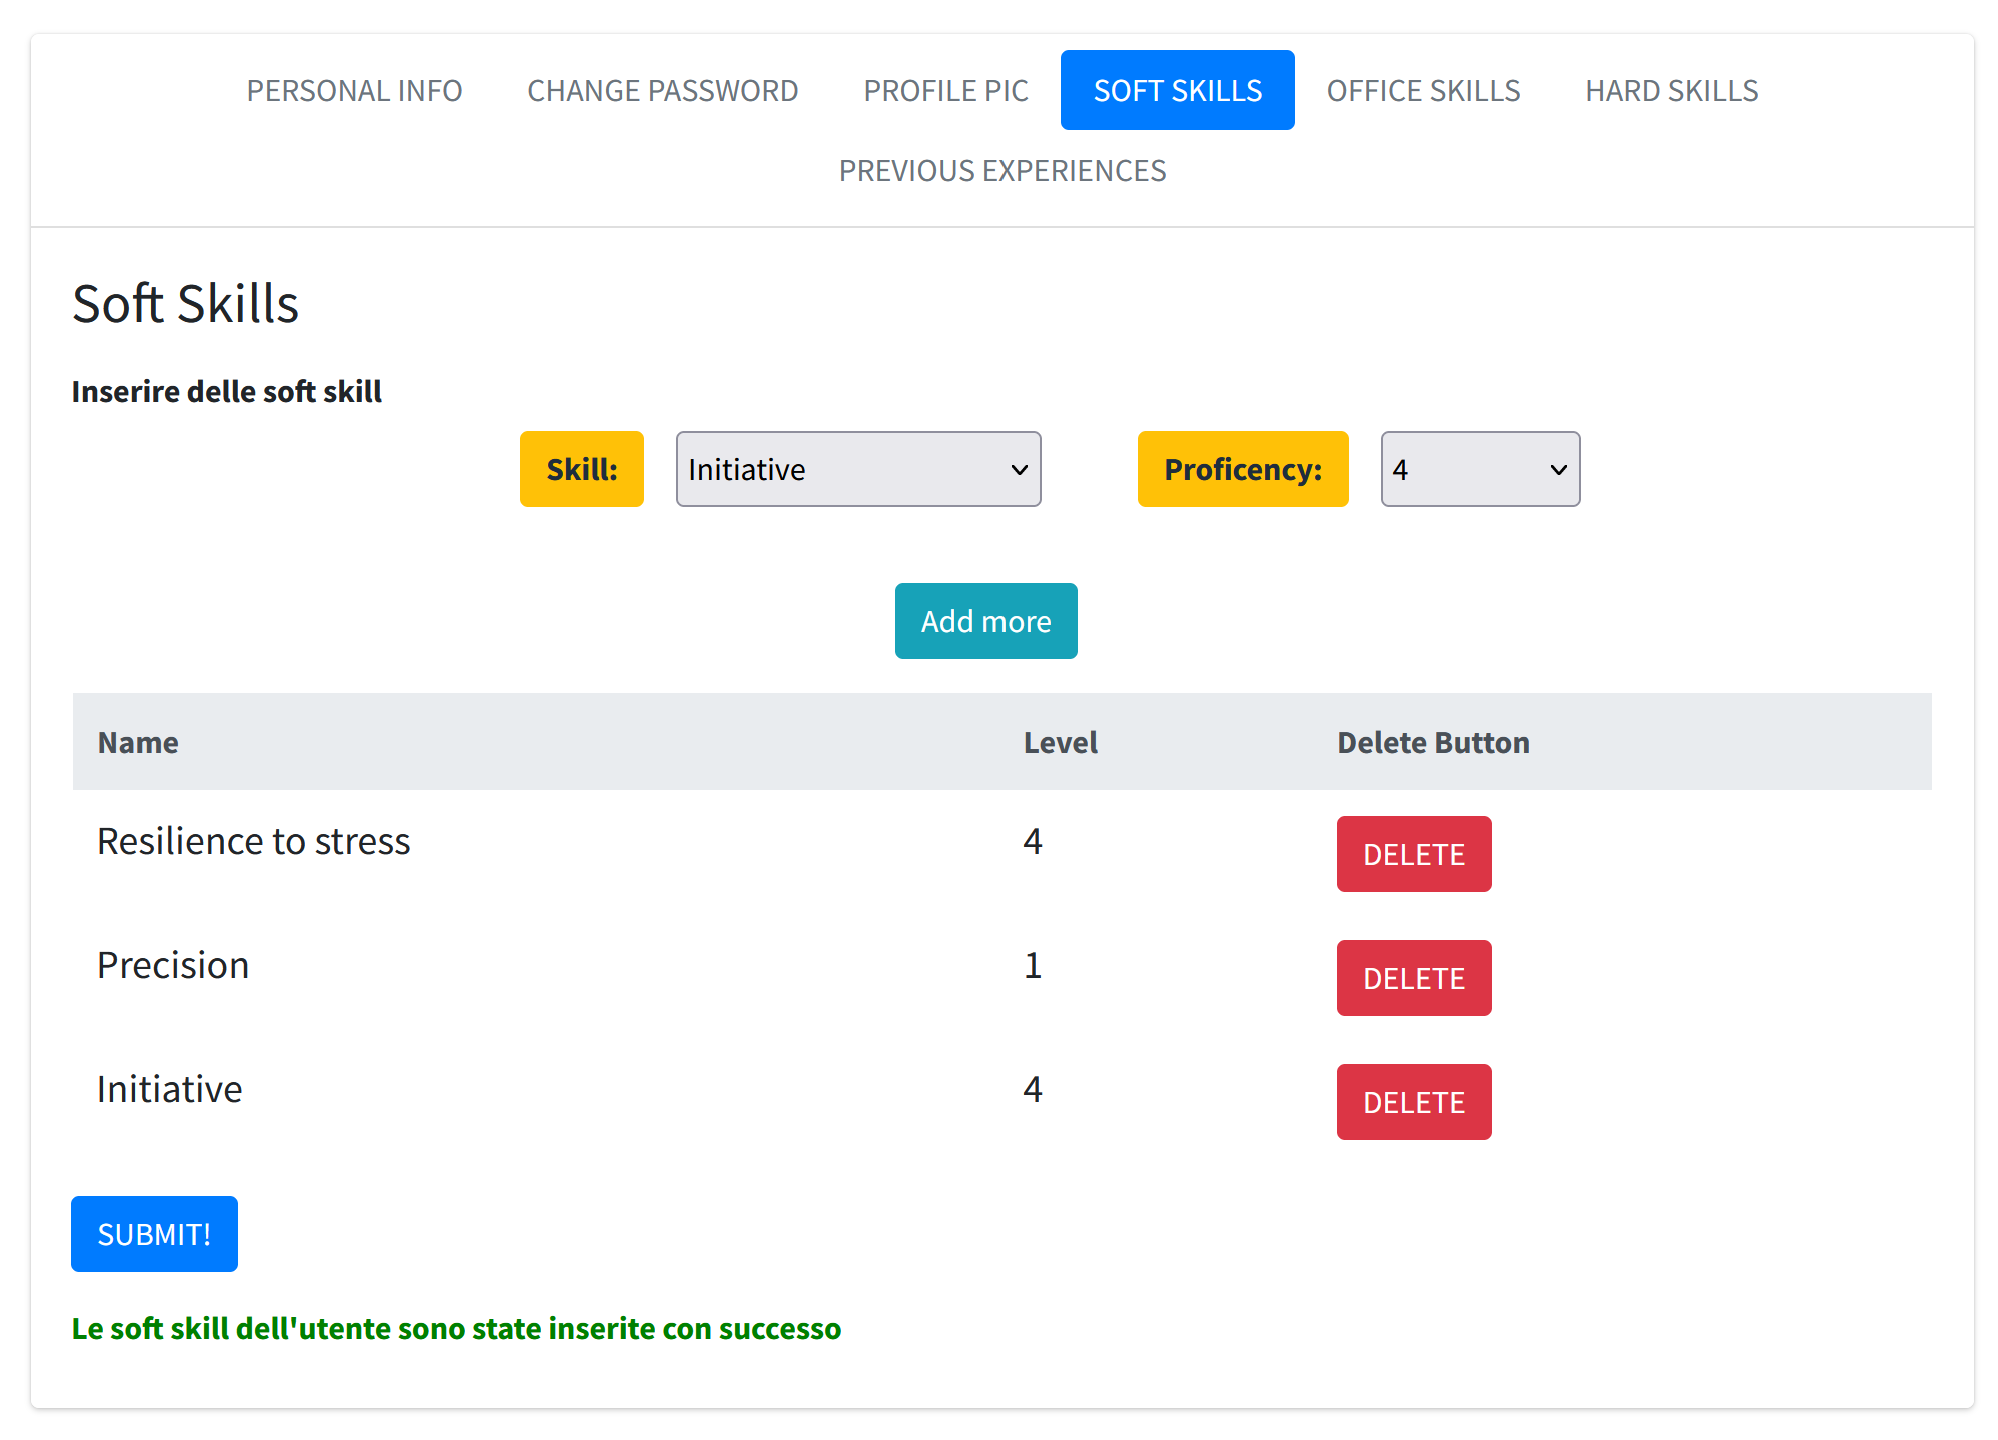
\includegraphics[width=450px]{./images/soft_skills.png}
        \caption{Sezione di modifica delle soft skill associate al proprio profilo}
        \label{fig:modificaInformazioni}
    \end{figure}
    
    \item Sezione di modifica delle office skills, la tecnica implementativa è identica a quella impiegata sulle soft skill.
    
    \item Sezione di modifica delle hard skills, mostrata in figura \ref{fig:hardSkills}.
    \\
    Per quello che riguarda le hard skills ho deciso di consentire l'inserimento libero delle informazioni da parte dell'utente, in quanto si tratta di un panorama talmente vasto e vario che andare a inserire le voci in un menu sarebbe stato troppo riduttivo. Maggiore libertà implica che vi saranno sicuramente degli abusi della feature, sarebbe infatti possibile per chiunque andare ad inserire delle skill che non hanno o che non esistono nemmeno.
    \\
    Siccome il sistema di valutazione è autogestito, il problema si ripercuote anche sulle soft skill e le skill del pacchetto Office. \'E  per questo che ho deciso di fare sì che gli admin abbiano la possibilità di modificare le skill di qualsiasi utente che abbia dei privilegi associati inferiori a quelli che possiedono loro. "Quis custodiet ipsos custodes?" A tal riguardo dedicherò una sezione in conclusione del capitolo.
    \\
    Comunque anche in questo caso la skill viene aggiunta a una lista temporanea tramite l'interazione con il pulsante "ADD" e viene successivamente caricata nel database dopo aver cliccato il pulsante "SUBMIT". \'E possibile andare a cancellare delle entry precedentemente inserite impiegando il pulsante di "DELETE".
    \begin{figure}[h]
        \centering
        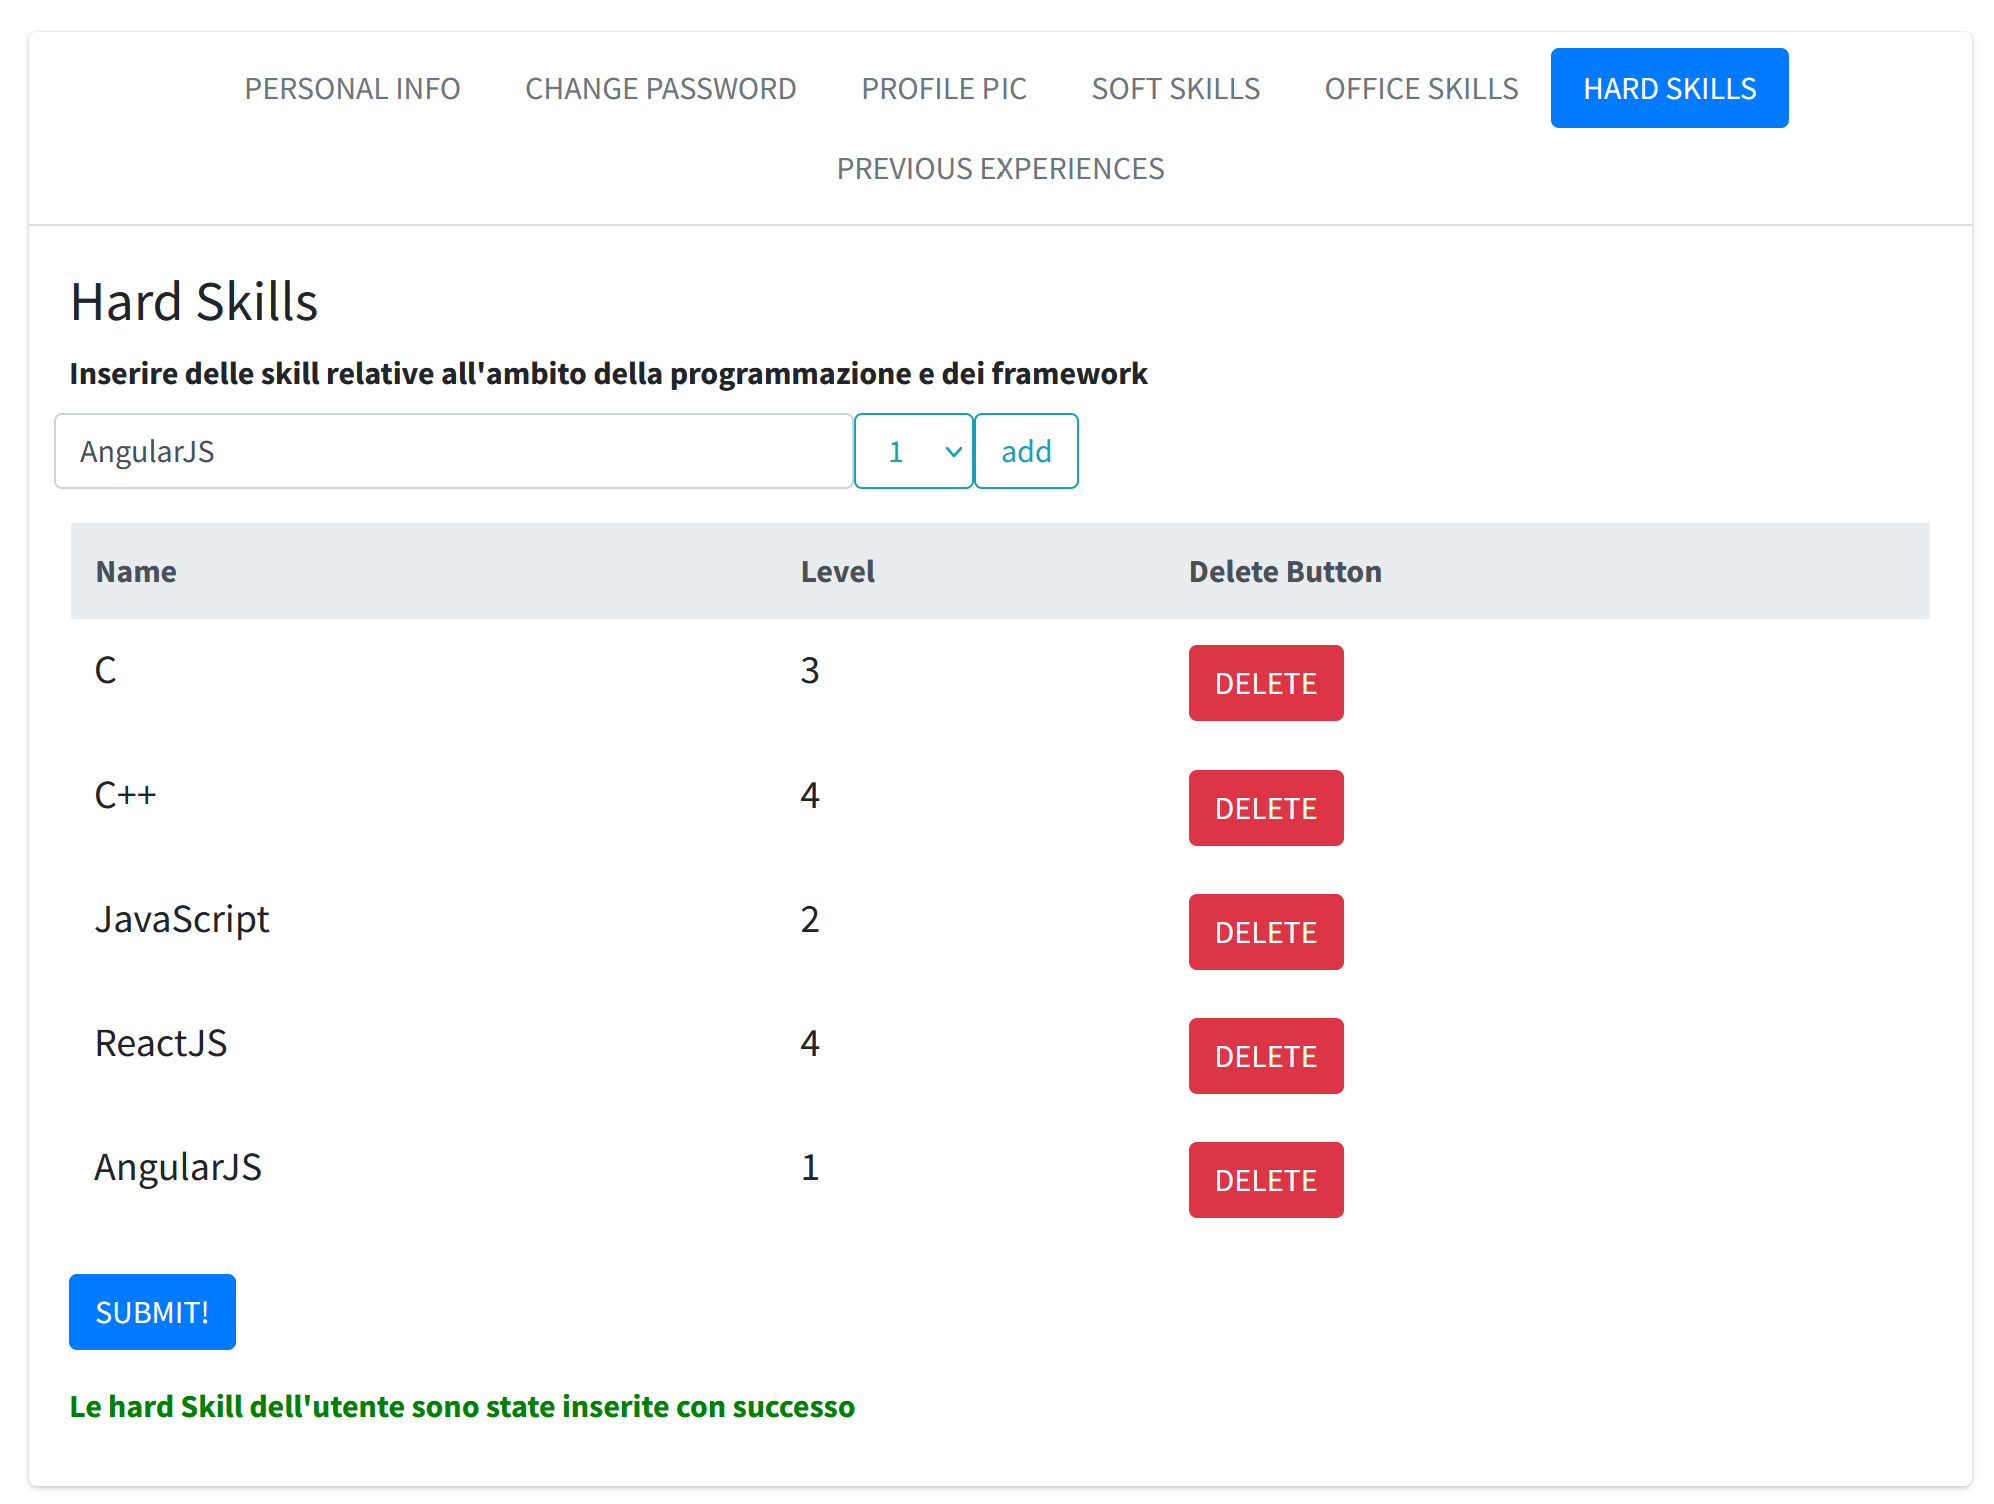
\includegraphics[width=450px]{./images/hard_skills.png}
        \caption{Sezione di modifica delle hard skill associate al proprio profilo}
        \label{fig:hardSkills}
    \end{figure}
    
    \item Sezione di modifica delle esperienze pregresse, questo menu consente di inserire le proprie esperienze lavorative. Su proposta del mio capo ho optato per inserirne di due tipi diversi:
    \begin{itemize}
        \item Le esperienze di lavoro, caratterizzate da:
        \begin{itemize}
            \item Una data di inizio
            \item Una data di fine
            \item Una società
            \item Una posizione
            \item Un resoconto dell'esperienza
        \end{itemize}
        \item Le esperienze di consulenza, durante le quali l'utente lavora presso Certimeter ma viene inviato come consulente presso un'azienda esterna, sono caratterizzate da:
        \begin{itemize}
            \item Una data di inizio
            \item Una data di fine
            \item Una posizione
            \item Una società
        \end{itemize}
        \'E possibile passare da un'esperienza di consulenza a un'esperienza lavorativa pregressa utilizzando l'apposito flag. Anche in questo caso l'esperienza viene aggiunta a una lista temporanea a seguito del click sul pulsante "ADD". Successivamente le modifiche vengono caricate nel database dopo che è stato premuto il pulsante "SUBMIT".
    \end{itemize}
\end{itemize}

%%%%%%%%%%%%%%%%%%%%%%%%%%%%%
\subsection{Admin functions}
%%%%%%%%%%%%%%%%%%%%%%%%%%%%%
La sezione di admin functions consente agli utenti che ne hanno i diritti di eseguire una serie di operazioni che coinvolgono gli utenti del sistema.
\begin{itemize}
    \item Visualizzazione di tutti gli utenti presenti nel database, per ciascun utente è possibile modificare le autovalutazioni (soft skill, hard skill, skill di office) perchè questo potrebbe essersi sopravvalutato o sottovalutato. \'E anche possibile visualizzarne i dati e abilitare/disabilitare l'utente per consentire/impedire l'accesso al sistema.
    \begin{figure}[h]
        \centering
        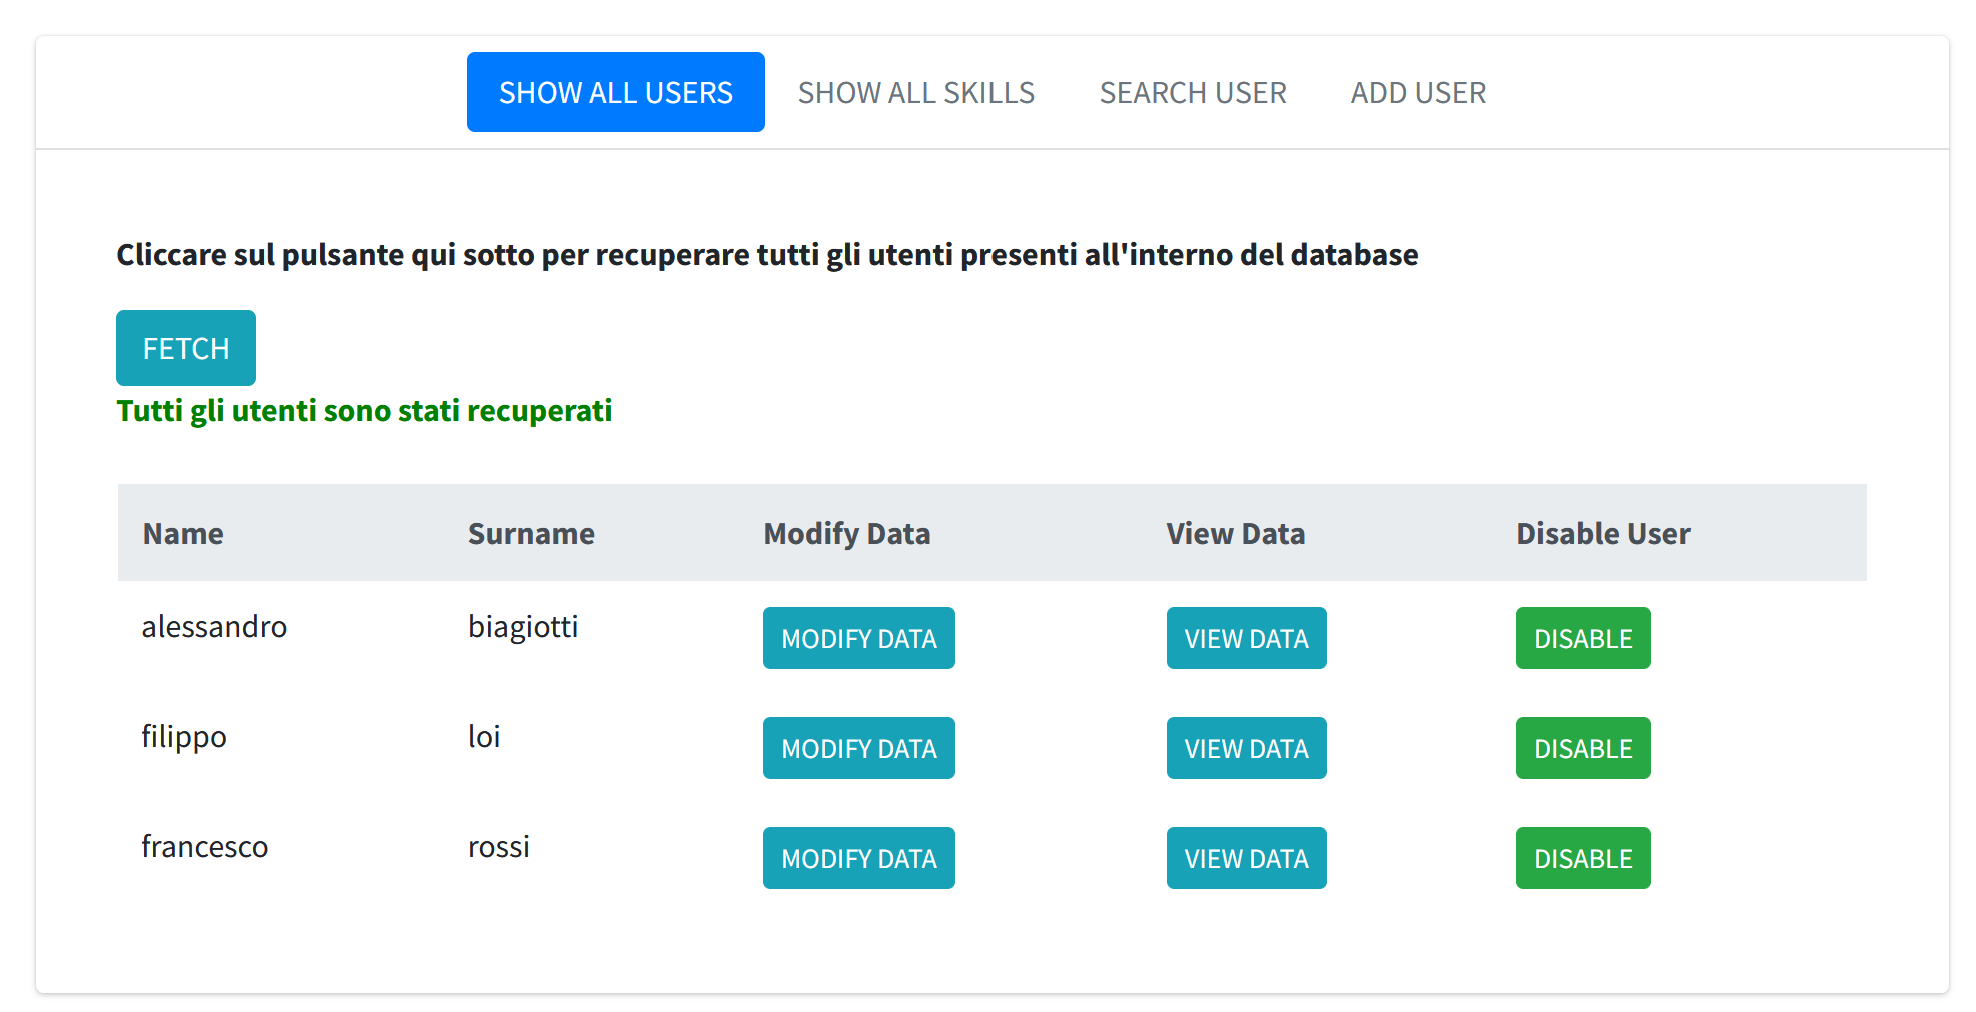
\includegraphics[width=450px]{./images/show_all_users.png}
        \caption{Sezione di visualizzazione di tutti gli utenti presenti nel database}
    \end{figure}
    \item Sezione di visualizzazione di tutte le skill presenti nel sistema.
    \item Sezione di ricerca di uno specifico utente presente nel sistema, la ricerca è eseguita impiegando la mail dell'utente.
    \item La sezione di inserimento di un nuovo utente, questa opzione controlla che la mail inserita sia della forma "nome.cognome@certimeter.it" e successivamente invia una mail a tale indirizzo indicando che l'utente è stato invitato ad entrare nel sistema.
    \\
    In allegato alla mail vengono inviati una password generata in maniera casuale (che si richiede di cambiare dopo il primo accesso) e il link di accesso all'applicazione.
    \\
    Un esempio di mail inviata all'utente può essere vista in figura \ref{fig:esempioMail}.
    \begin{figure}[h]
        \centering
        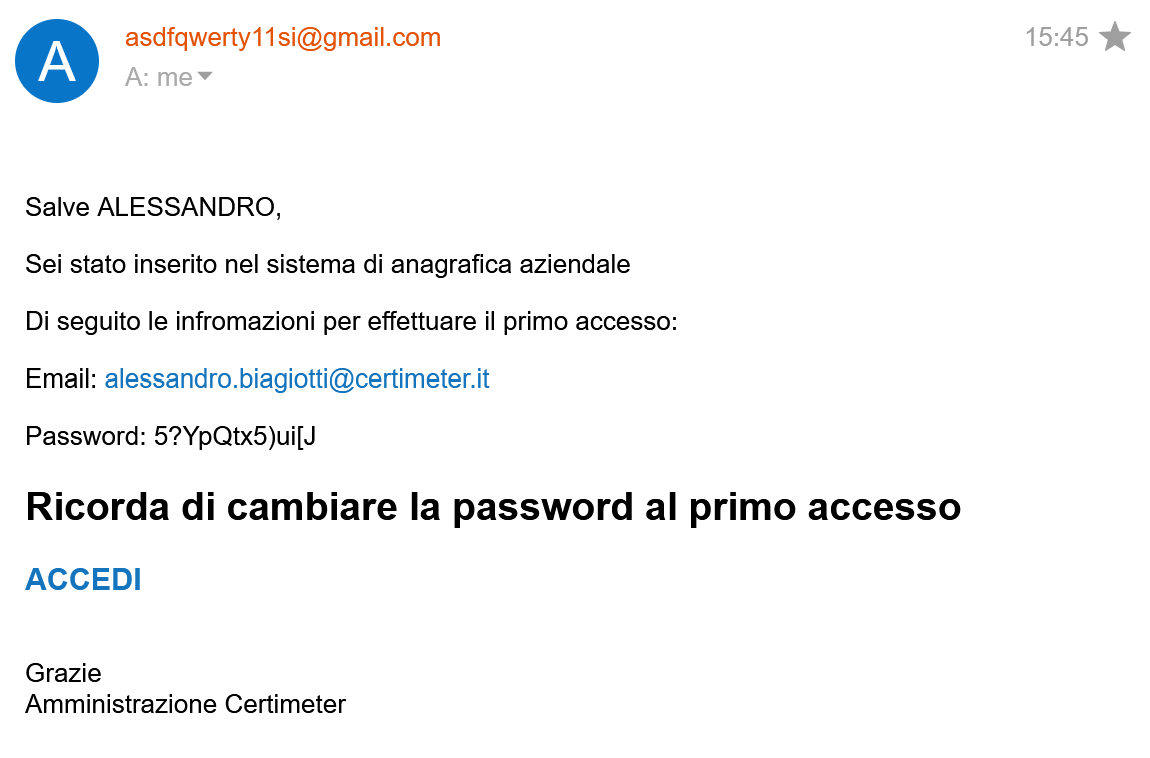
\includegraphics[width=300px]{./images/mail_conferma.png}
        \caption{esempio di mail di conferma}
        \label{fig:esempioMail}
    \end{figure}
\end{itemize}

%%%%%%%%%%%%%%%%%%%%%%%%%%%%%
\subsection{Logout}
%%%%%%%%%%%%%%%%%%%%%%%%%%%%%
La sezione di Logout non è, di per se, particolarmente interessante. L'utente ha la possibilità di uscire dall'applicazione impiegando l'apposito tasto rosso "LOG ME OUT". Ovviamente tutte le informazioni contenute all'interno dello storage del browser vengono eliminate una volta che l'utente esce.

%%%%%%%%%%%%%%%%%%%%%%%%%%%%%
\section{Altri utenti}
%%%%%%%%%%%%%%%%%%%%%%%%%%%%%
Come anticipavo in precedenza, gli admin nel sistema hanno il controllo quasi assoluto delle informazioni tecniche degli utenti, ovviamente la feature è stata pensata con intento benigno perchè vi è la necessità di un qualche genere di moderazione sulle autovalutazioni. Al tempo stesso, però, il sistema cela una grossa problematica: gli admin possono modificare le informazioni degli utenti, ma nessuno può modificare le informazioni degli admin (ho evitato di inserire il controllo tra admin per ovvie ragioni).
\\
\'E proprio a questo che serve l'utente superAdmin, la cui interfaccia utente viene mostrata nella figura \ref{fig:homepageSuperAdmin}.
\\
Dato che il superAdmin non è un utente normale, ma un costrutto, ho deciso di togliere qualsiasi cosa potesse indicare che si tratti di una persona e lasciare solamente le funzionalità strettamente necessarie.
\begin{figure}[h]
    \centering
    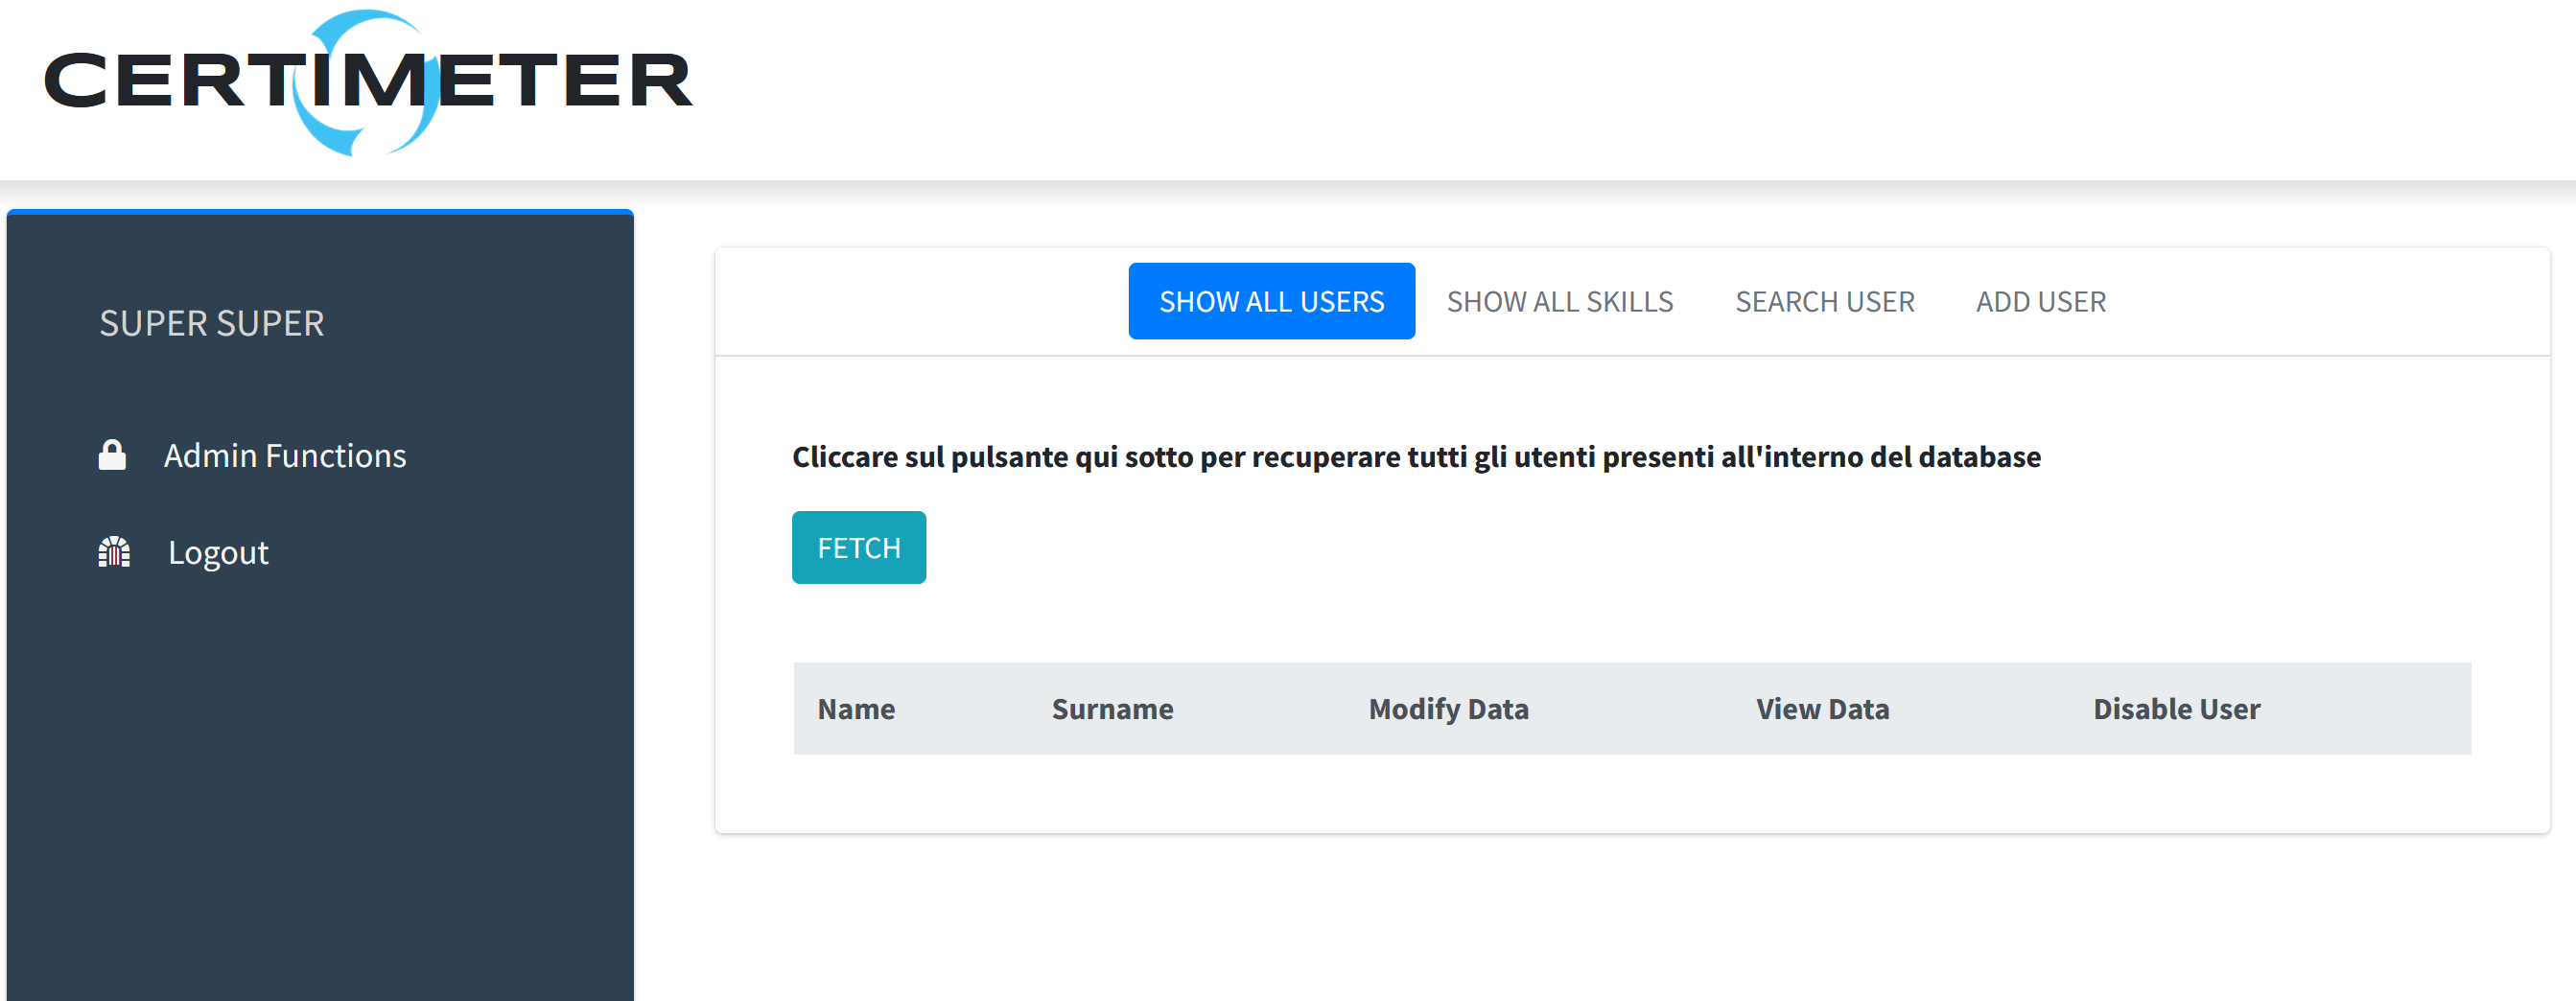
\includegraphics[width=450px]{./images/super_admin.png}
    \caption{la struttura dell'interfaccia di un superadmin}
    \label{fig:homepageSuperAdmin}
\end{figure}
La struttura del menu di amministrazione del superAdmin è la stessa del menu dell'admin. Gli unici cambiamenti sono nella logica. La voce "SHOW ALL USERS" mostra unicamente gli admin presenti nel sistema, così da poter agire più rapidamente sul target per cui è stato specificamente costruito. Sebbene il principale obiettivo del superAdmin sia quello di "controllare i controllori" riesce ad agire direttamente anche sugli utenti normali tramite la voce "SEARCH ALL USER".